%%%%%%%%%%%%%%%%%%%%%%%%%%%%%%%%%%%%%%%%%
% Lachaise Assignment
% LaTeX Template
% Version 1.0 (26/6/2018)
%
% This template originates from:
% http://www.LaTeXTemplates.com
%
% Authors:
% Marion Lachaise & François Févotte
% Vel (vel@LaTeXTemplates.com)
%
% License:
% CC BY-NC-SA 3.0 (http://creativecommons.org/licenses/by-nc-sa/3.0/)
% 
%%%%%%%%%%%%%%%%%%%%%%%%%%%%%%%%%%%%%%%%%

%----------------------------------------------------------------------------------------
%	PACKAGES AND OTHER DOCUMENT CONFIGURATIONS
%----------------------------------------------------------------------------------------

\documentclass{article}

\usepackage{dirtree}
\usepackage{hyperref}
\usepackage{comment}
\usepackage{caption}

%%%%%%%%%%%%%%%%%%%%%%%%%%%%%%%%%%%%%%%%%
% Lachaise Assignment
% Structure Specification File
% Version 1.0 (26/6/2018)
%
% This template originates from:
% http://www.LaTeXTemplates.com
%
% Authors:
% Marion Lachaise & François Févotte
% Vel (vel@LaTeXTemplates.com)
%
% License:
% CC BY-NC-SA 3.0 (http://creativecommons.org/licenses/by-nc-sa/3.0/)
% 
%%%%%%%%%%%%%%%%%%%%%%%%%%%%%%%%%%%%%%%%%

%----------------------------------------------------------------------------------------
%	PACKAGES AND OTHER DOCUMENT CONFIGURATIONS
%----------------------------------------------------------------------------------------

\usepackage{amsmath,amsfonts,stmaryrd,amssymb} % Math packages

\usepackage{enumerate} % Custom item numbers for enumerations

\usepackage[ruled]{algorithm2e} % Algorithms

\usepackage[framemethod=tikz]{mdframed} % Allows defining custom boxed/framed environments

\usepackage{listings} % File listings, with syntax highlighting
\lstset{
	basicstyle=\ttfamily, % Typeset listings in monospace font
}

%----------------------------------------------------------------------------------------
%	DOCUMENT MARGINS
%----------------------------------------------------------------------------------------

\usepackage{geometry} % Required for adjusting page dimensions and margins

\geometry{
	paper=a4paper, % Paper size, change to letterpaper for US letter size
	top=2.5cm, % Top margin
	bottom=3cm, % Bottom margin
	left=2.5cm, % Left margin
	right=2.5cm, % Right margin
	headheight=14pt, % Header height
	footskip=1.5cm, % Space from the bottom margin to the baseline of the footer
	headsep=1.2cm, % Space from the top margin to the baseline of the header
	%showframe, % Uncomment to show how the type block is set on the page
}

%----------------------------------------------------------------------------------------
%	FONTS
%----------------------------------------------------------------------------------------

\usepackage[utf8]{inputenc} % Required for inputting international characters
\usepackage[T1]{fontenc} % Output font encoding for international characters

\usepackage{XCharter} % Use the XCharter fonts

%----------------------------------------------------------------------------------------
%	COMMAND LINE ENVIRONMENT
%----------------------------------------------------------------------------------------

% Usage:
% \begin{commandline}
%	\begin{verbatim}
%		$ ls
%		
%		Applications	Desktop	...
%	\end{verbatim}
% \end{commandline}

\mdfdefinestyle{commandline}{
	leftmargin=10pt,
	rightmargin=10pt,
	innerleftmargin=15pt,
	middlelinecolor=black!50!white,
	middlelinewidth=2pt,
	frametitlerule=false,
	backgroundcolor=black!5!white,
	frametitle={Command Line},
	frametitlefont={\normalfont\sffamily\color{white}\hspace{-1em}},
	frametitlebackgroundcolor=black!50!white,
	nobreak,
}

% Define a custom environment for command-line snapshots
\newenvironment{commandline}{
	\medskip
	\begin{mdframed}[style=commandline]
}{
	\end{mdframed}
	\medskip
}

%----------------------------------------------------------------------------------------
%	FILE CONTENTS ENVIRONMENT
%----------------------------------------------------------------------------------------

% Usage:
% \begin{file}[optional filename, defaults to "File"]
%	File contents, for example, with a listings environment
% \end{file}

\mdfdefinestyle{file}{
	innertopmargin=1.6\baselineskip,
	innerbottommargin=0.8\baselineskip,
	topline=false, bottomline=false,
	leftline=false, rightline=false,
	leftmargin=2cm,
	rightmargin=2cm,
	singleextra={%
		\draw[fill=black!10!white](P)++(0,-1.2em)rectangle(P-|O);
		\node[anchor=north west]
		at(P-|O){\ttfamily\mdfilename};
		%
		\def\l{3em}
		\draw(O-|P)++(-\l,0)--++(\l,\l)--(P)--(P-|O)--(O)--cycle;
		\draw(O-|P)++(-\l,0)--++(0,\l)--++(\l,0);
	},
	nobreak,
}

% Define a custom environment for file contents
\newenvironment{file}[1][File]{ % Set the default filename to "File"
	\medskip
	\newcommand{\mdfilename}{#1}
	\begin{mdframed}[style=file]
}{
	\end{mdframed}
	\medskip
}

%----------------------------------------------------------------------------------------
%	NUMBERED QUESTIONS ENVIRONMENT
%----------------------------------------------------------------------------------------

% Usage:
% \begin{question}[optional title]
%	Question contents
% \end{question}

\mdfdefinestyle{question}{
	innertopmargin=1.2\baselineskip,
	innerbottommargin=0.8\baselineskip,
	roundcorner=5pt,
	nobreak,
	singleextra={%
		\draw(P-|O)node[xshift=1em,anchor=west,fill=white,draw,rounded corners=5pt]{%
		Question \theQuestion\questionTitle};
	},
}

\newcounter{Question} % Stores the current question number that gets iterated with each new question

% Define a custom environment for numbered questions
\newenvironment{question}[1][\unskip]{
	\bigskip
	\stepcounter{Question}
	\newcommand{\questionTitle}{~#1}
	\begin{mdframed}[style=question]
}{
	\end{mdframed}
	\medskip
}

%----------------------------------------------------------------------------------------
%	WARNING TEXT ENVIRONMENT
%----------------------------------------------------------------------------------------

% Usage:
% \begin{warn}[optional title, defaults to "Warning:"]
%	Contents
% \end{warn}

\mdfdefinestyle{warning}{
	topline=false, bottomline=false,
	leftline=false, rightline=false,
	nobreak,
	singleextra={%
		\draw(P-|O)++(-0.5em,0)node(tmp1){};
		\draw(P-|O)++(0.5em,0)node(tmp2){};
		\fill[black,rotate around={45:(P-|O)}](tmp1)rectangle(tmp2);
		\node at(P-|O){\color{white}\scriptsize\bf !};
		\draw[very thick](P-|O)++(0,-1em)--(O);%--(O-|P);
	}
}

% Define a custom environment for warning text
\newenvironment{warn}[1][Warning:]{ % Set the default warning to "Warning:"
	\medskip
	\begin{mdframed}[style=warning]
		\noindent{\textbf{#1}}
}{
	\end{mdframed}
}

%----------------------------------------------------------------------------------------
%	INFORMATION ENVIRONMENT
%----------------------------------------------------------------------------------------

% Usage:
% \begin{info}[optional title, defaults to "Info:"]
% 	contents
% 	\end{info}

\mdfdefinestyle{info}{%
	topline=false, bottomline=false,
	leftline=false, rightline=false,
	nobreak,
	singleextra={%
		\fill[black](P-|O)circle[radius=0.4em];
		\node at(P-|O){\color{white}\scriptsize\bf i};
		\draw[very thick](P-|O)++(0,-0.8em)--(O);%--(O-|P);
	}
}

% Define a custom environment for information
\newenvironment{info}[1][Info:]{ % Set the default title to "Info:"
	\medskip
	\begin{mdframed}[style=info]
		\noindent{\textbf{#1}}
}{
	\end{mdframed}
}
 % Include the file specifying the document structure and custom commands

%----------------------------------------------------------------------------------------
%	ASSIGNMENT INFORMATION
%----------------------------------------------------------------------------------------

\title{Networking and Remote Services with\\ RU-Store: A Remote Object Store} % Title of the assignment

%\author{Yukiko Amagi\\ \texttt{y.amagi@inabauniversity.jp}} % Author name and email address


%\author{Rutgers University} % Author name and email address

\date{}%Due: October 17, 11:55pm} % University, school and/or department name(s) and a date

%----------------------------------------------------------------------------------------

\begin{document}

\maketitle % Print the title

%----------------------------------------------------------------------------------------
%	INTRODUCTION
%----------------------------------------------------------------------------------------

\vspace{-1.5cm}

\section*{Introduction} % Unnumbered section
Distributed systems and services are a great way to expand the amount of computation power and storage capacity used by an application beyond that of a single system. However, before we can explore more advanced distributed systems concepts and complexities, we should first refresh and understand the complexity of building a simple service that can be used in a distributed setting.

In this project you will be exploring the complexities of client-server communication and refreshing your network programming skills by implementing your own remote object store from the ground up. By the end of this project you would have implemented your own server and client library, designed your own communication protocol to transfer information between the two, as well as learned a thing or two about modern storage services.


%----------------------------------------------------------------------------------------
%	Section 
%----------------------------------------------------------------------------------------

\section{Background: Object Stores} % Numbered section
Modern social media services and applications have become more data driven, generating large amounts of data not only for media hosting but for analytics. It has been harder to find proper storage solutions to store arbitrary, unstructured data. File systems can be used to store such data within a file system tree, however, maintaining a proper file system tree becomes burdensome and the amount of file metadata (attributes that describe the contents) that can be stored for each file is limited by the file system.
 
To allow for better scaling of storing unstructured data, object-based stores have been developed. In this case any kind of data be stored as an object, from a string, to pictures, to videos. Within an object store, objects are stored in a flat namespace using a unique identifier or key. This removes the need to organize and maintain some data hierarchy. Along with each piece of data, a piece of metadata can also be attached for each object to allow for an arbitrary amount of metadata to be stored. This allows better flexibility in terms of storing contextual information about the file compared to other forms of storage.  

Because of these benefits, object storage has become more popular with cloud services like Amazon S3, Google Cloud, and Microsoft Azure providing remote object storage to allow for clients (such as social media services) to store large amounts of data and objects in the cloud. Other popular storage solutions such Ceph, allows for clients to scale object storage on their own infrastructure and is used in private and high performance computing environments. 

\-\ \\ \noindent \textbf{You can read more about object stores here:}
\href{https://en.wikipedia.org/wiki/Object_storage}{https://en.wikipedia.org/wiki/Object\_storage}

\begin{figure}[hbt!]
\vspace{-0.0cm}
\includegraphics[width=14cm]{images/cloudobjectstores}
\centering
\caption{Popular Cloud-based Object Storage Solutions}
\end{figure}



%----------------------------------------------------------------------------------------
\section{Architecture and Design}

%----------------------------------------------------------------------------------------
In order to implement your own object store, there will be two things you will have to implement: (1) the RUStore client library and (2) the RUStore Server. The client library is the interface the user application will use to interact and pass information between the application and the object store server. 

\begin{figure}[h]
\vspace{0.2cm}
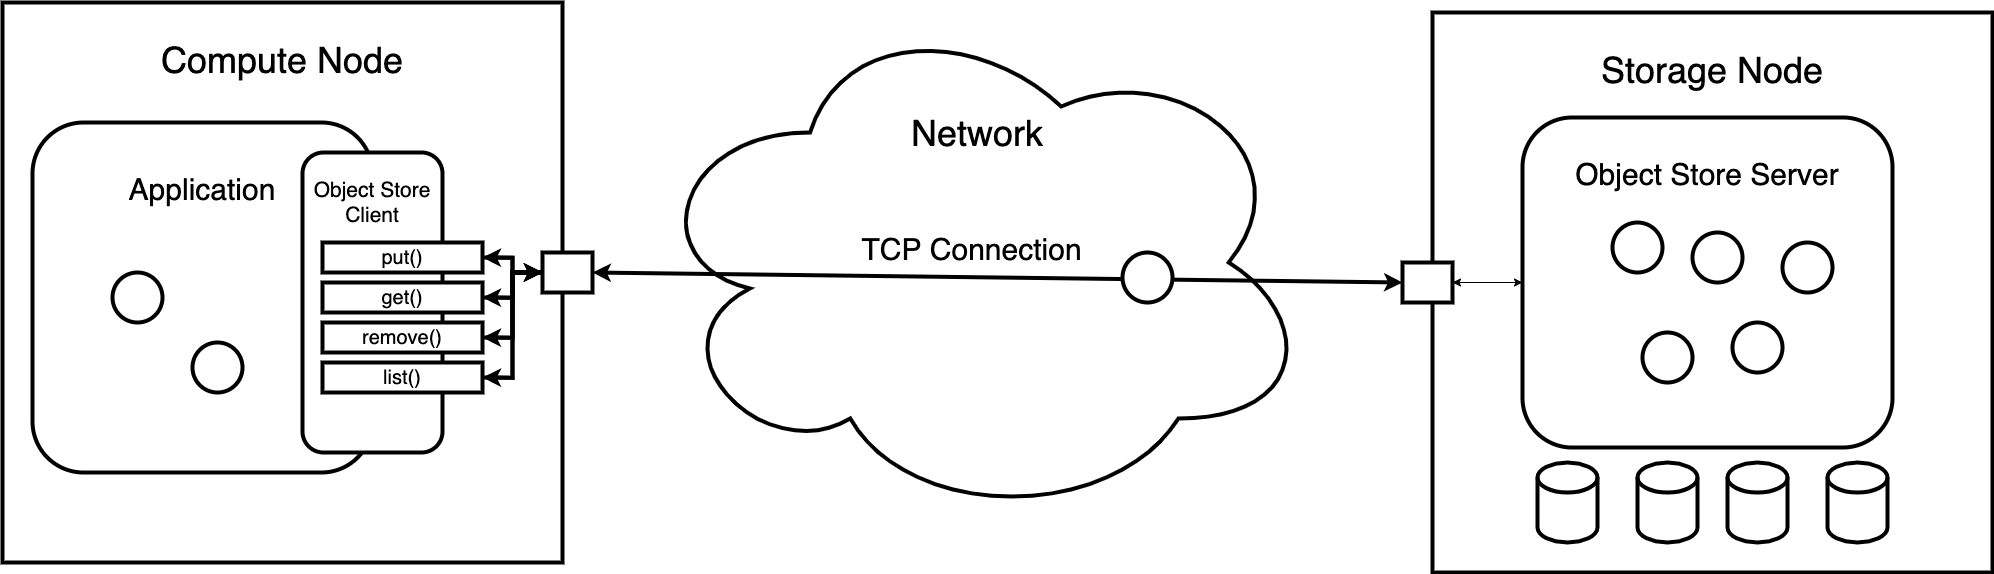
\includegraphics[width=16cm]{images/objectstore.png}
\centering
\caption{Object Store Architecture}
\vspace{-0.3cm}
\end{figure}

\subsection*{RUStore Client}
In order to interact with a remote RUStore Server, an application must create an RUStore Client. Using the RUStore Client, the application is then able to connect to the remote RUStore Server. The application can then use the client methods perform object store operations. \\

\noindent Within the client class \textit{RUStoreClient.java} you will have to implement the following methods: 
\begin{itemize}
    %\item \textbf{connect(String host, int port)}
    \item \textbf{RUStoreClient(String host, int port)} \vspace{0.1cm} \\ 
            Constructor that initializes client object to be used to communicate with the remote object server. 
    \item \textbf{void connect()} \vspace{0.1cm} \\
            Creates a socket and opens up a connection to the remote object server.
    \item \textbf{int put(String key, byte[] data)} \vspace{0.1cm} \\ 
            Sends a data object represented by an array of bytes to the object 
            server which will store the data with a given key. This is useful for offloading data stored within memory such as computational results or application objects that you don't want to persist locally. 
    \item \textbf{int put(String key, String file\_path)} \vspace{0.1cm} \\
            Sends data from a file to the object server which will store the data with a given key. This is useful for offloading and distributing large binary files stored locally such as videos, images, etc. \textit{Note how this is similar to put(String key, byte[]), except that the bytes are coming from a file instead.}
    \item \textbf{byte[] get(String key)} \vspace{0.1cm} \\
            Downloads an object associated with a given key and returns the data as a byte array. This is useful for downloading data objects that you don't necessarily want to persist. For example you may want to download some results of data to perform quick processing and computation on.
    \item \textbf{int get(String key, String file\_path)} \vspace{0.1cm} \\
            Downloads object associated with a given key and writes it to a specified file. This is useful for downloading large data objects that may be too unwieldy to keep around in memory such as videos or compressed files or any data that you want to process at a later time. \textit{Note how this is similar to get(String key), except that bytes are should be directed to a file instead of a byte array in memory.}
    \item \textbf{int remove(String key)} \vspace{0.1cm} \\
            Removes an object from the object server. Note that this doesn't download the object, it simply tells the object store to free the object on the server side. 
    \item \textbf{String[] list()} \vspace{0.1cm} \\
            Fetches a list of all object keys from the object store and returns them as a list of String objects.
    %\item \textbf{stat(key)} - get object metadata
    \item \textbf{void disconnect()} \vspace{0.1cm} \\
            Sends a message to the server to inform the connection will close so the server socket can be closed gracefully. After sending the server a message, it closes the client socket and connection. 
            
\end{itemize}

\noindent \textbf{Note:} To see more details such as what kind of situations you should handle and what are the valid return values for each method, please take a look at the Java documentation within \textit{RUStoreClient.java}.

\subsection*{RUStore Server}
The RUStore Server a runnable java program that will need to be implemented in the server class\\ \textit{RUStoreServer.java}. The RUStoreServer class is empty besides the main() method. The main method accepts a single argument which is the port number the server should run on. You will have to add any necessary classes, add any static members, as well as any helper methods to help implement the server program. 



%----------------------------------------------------------------------------------------
%	Section 
%----------------------------------------------------------------------------------------

\section{Project Stages} % Numbered section

To implement our Remote Object Store, we break down this project into four stages designed to help with incremental implementation:
\begin{itemize}  
\item \textbf{Stage 1} – Building a Connection
\item \textbf{Stage 2} – Implementing a Communication Protocol
\item \textbf{Stage 3} – Passing Arbitrary Objects and Files
\item \textbf{Stage 4} – Object Storage
\end{itemize}

\begin{comment}
\begin{info}[Note:]
It is not required to follow these stages exactly. You are free to implement the program with whatever approach you want. These stages are mainly designed for those that are either relatively new to network programming or those who a little bit rusty and would prefer to ease into it.
\end{info}
\end{comment}

%---------------------------------------------------------------------------------------


%----------------------------------------------------------------------------------------
%	Section 
%----------------------------------------------------------------------------------------

\section{Stage 1: Building a Connection} % Numbered section


\begin{large}\textbf{Goal:}\end{large} Build a simple connection between a client and server and pass basic information between\\ \indent \indent \-\ the two.

\begin{figure}[h]
\vspace{0.2cm}
\hspace{-0.8cm}
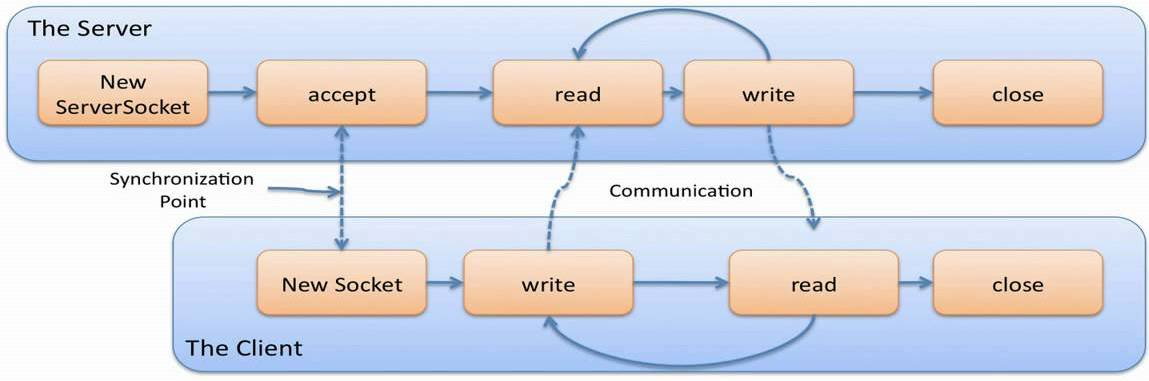
\includegraphics[width=14cm]{images/javasocket}
\centering
\caption{Basic Socket Communication Flow}
\vspace{-0.3cm}
\end{figure}

\subsection*{Overview:}
Before we can start passing things, we will need to start off by making a connection and start to learn how to pass information back and forth between the client and server. This will require to do the following things:
\begin{enumerate}
    \item On the server, open a socket and bind it to a port to start listening for incoming connections.
    \item On the client, open a socket and establish a connection to the remote server. 
    \item Use read() and write() to send and receive data between the client and server.
    \item Close the connection and sockets on both the client and server when messages are done being passed. 
\end{enumerate}

\subsection*{Approach:}
In order to implement this within you client and server you will need know how to use Java Sockets and Input/Output Streams. Before starting your implementation within the RUStoreClient and RUStoreServer classes, first build simple client and server programs outside to the project by looking at the following references and guides:

\begin{itemize}
    \item \textbf{Network Programming Slides.} See lecture slides on Canvas
    \item \textbf{A Guide to Java Sockets.} \href{https://www.baeldung.com/a-guide-to-java-sockets}{https://www.baeldung.com/a-guide-to-java-sockets}
\end{itemize}

\noindent One you get the hang of simple of how to use sockets and streams, you can start to implementing the client and server logic within the following places:

\begin{enumerate}
    \item \textbf{RUStoreClient.java}
        \begin{itemize}
            \item RUStoreClient() constructor
            \item int connect()
            \item int disconnect()
        \end{itemize}
    \item \textbf{RUStoreServer.java}
        \begin{itemize}
            \item void main()
        \end{itemize}
\end{enumerate}



\subsection*{Testing:}
Testing your implementation with the client and server requires both to be running. Running the\\ RUStoreServer should be easy and straight forward. However, running the RUStoreClient is not as it's simply a client library that is used by applications. 

To test if the RUStoreClient works with the basic client logic you implemented so far, use the Sandbox program (\textit{TestSandbox.java}) to create a RUStoreClient object and call the connect() and disconnect() methods. To see more on how to build and run your programs including the sandbox program, take a look at Section \ref{section:build} and \ref{section:run}.

\subsection*{Other Notes:}
\begin{info}[Handling Exceptions.]
As you start to fill in the client methods, you'll notice that certain libraries/packages you use can potentially throw exceptions and cause an issue. For example, when using the java.net package, if you try and open a connection and the host is not valid, an \textit{UnknownHostException} would be thrown. In this case you should throw the exception from the client method so the calling application can handle it accordingly like:\\

\vspace{-0.2cm}
\indent void connect() \textbf{throws UnknownHostException}\{...\}\\
\vspace{-0.2cm}

\noindent Do avoid throwing the generic Exception to handle all exceptions like: \\

\vspace{-0.2cm}
\indent void connect() \textbf{throws Exception}\{...\} \\
\vspace{-0.2cm}

\noindent Allowing a method to throw a generic exception is not good practice as any application utilizing the library will be unaware of what kind of exception it is (ex. i/o exception, unknown host exception, etc...) and will have to look into the exception details in order to figure out what to do next. It's best to list out all the specific types of exceptions a method can throw to let users of the methods know what kind of errors they should expect to possibly handle.
\end{info}






%----------------------------------------------------------------------------------------

%----------------------------------------------------------------------------------------
%	Section 
%----------------------------------------------------------------------------------------

\section{Stage 2: Implementing the Communication Protocol} % Numbered section

\begin{large}\textbf{Goal:}\end{large} Design and implement your own communication protocol to allow for our client and server to\\ \indent \indent \-\ effectively communicate and understand data being sent back and forth.

\begin{figure}[h]
\vspace{0.2cm}
\hspace{-0.8cm}
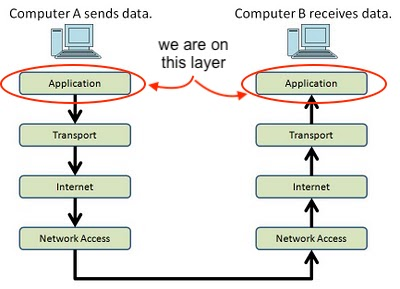
\includegraphics[width=10cm]{images/networking}
\centering
\captionsetup{justification=centering}
\caption{Data flow through the TCP/IP stack between 2 computers.\\Red shows the layer our protocol will reside in.}
\label{fig:networking}
%\vspace{-0.3cm}
\end{figure}

\subsection*{Overview:}

\begin{comment}
\textbf{The layers of communication.} As shown in figure \ref{fig:networking}, there are multiple layers data has to pass through to get to reach its destination. You don't need to know the specific details and roles of each layer, but just know that each layer works together to ensure data is sent to the right place in a reliable manner. \\ 
\end{comment}

\noindent \underline{\textbf{Need for a higher level protocol}} \vspace{0.2cm} \\
In the previous stage, you used Java sockets to open a TCP connection. The TCP protocol exists on the transport layer and provides enough capability to reliably transfer data over the network. However at this point, how does an application know to interpret the data being received? Further, how does it know what kind of data to send back and when?

This is where the application layer comes in. Protocols existing on the application layer utilize lower level protocols (like TCP) to send data over the network while helping applications effectively exchange data by defining how the endpoints should communicate and what kind of data they should expect to send and receive. This is where we currently stand in our project. \\

\noindent \underline{\textbf{Why need your own protocol?}} \vspace{0.2cm} \\
We know at this point we need a higher level protocol to allow for our client and server to communicate effectively. We could perhaps use existing communication protocols such as HTTP. However, despite being widely used, there would be extra bulk when using it, since it has more functionality than we actually need. In light of low networking latencies and data generation increasing, it would be better for us to come up with our own simple and lightweight protocol to maximize performance and data throughput.\\ 

\noindent \underline{\textbf{Towards designing our own protocol}} \vspace{0.2cm} \\
\noindent When designing your communication protocol, you will need to consider a couple things:
\begin{itemize}
    \item \textbf{Message Types.} Remember, for each of the client methods you will want the server to perform different actions, so you must format the messages being sent from the client in such as way where the server can understand what kind of data is in the message and what kind of action it should take.
    \item \textbf{Special Response Messages.} After sending a request message, the client should wait for a response from the server to ensure the server received and processed its message. Should a response message use the same format as the request messages coming from the server?
    \item \textbf{Variable Sized Messages.} You can assume keys when serialized won't be more than 1KB or 1024 bytes, however remember that data objects being sent over the network can be of any size. How can you account for this in your protocol?
\end{itemize}

\begin{comment}
You can read more about it here: \href{https://en.wikipedia.org/wiki/Internet_protocol_suite}{https://en.wikipedia.org/wiki/Internet\_protocol\_suite}

You can read more about the application layer here: \href{https://en.wikipedia.org/wiki/Application_layer}{https://en.wikipedia.org/wiki/Application\_layer}
\end{comment}




\subsection*{Approach:}
If we start trying to take bytes representing different parts of our message, jam them together and start sending them it over the network hoping it will just work, chances are that it won't. Instead you should work to incrementally build your message protocol. \\

\begin{enumerate} 
    \item \textbf{Start with a simple message.} For example, start on incrementally building requests (messages from the client to the server). You can start off by sending a simple message encoding what kind of request it is (e.g put, get, ..). Then, on the server side, make sure you can properly receive the request and decipher what kind of request it is, printing out "put", "get", etc. depending on the message received. \\
    \item \textbf{Incrementally Build Add More To The Message.} After you do that, simply append more information to the end of the message. Try to append a key to the message and verify on the server side that you can properly decipher the longer message by not only printing out the request type, but also the key. \\
    \item \textbf{Figure out how to add arbitrary amounts of data} Once you get the hang of generating the messages and deciphering it on the other end, now its just a matter or designing the message in such a way to attach an arbitrary amount of data to it.\\ 
    \item \textbf{Repeat the same approach for other kinds of messages} After you finish designing and implementing client request messages, you can now use the same approach to design and implement server responses. 
\end{enumerate}

\noindent After figuring out the design and implementing message building, you can start populating and testing all the client methods, formatting messages with the required information for the operation (ignoring the object data), sending the message, and waiting for a response. You can also ensure that your server implementation is structured to handle every type of message and sends a response back to the client for any message it receives. 

\begin{comment}
\subsection*{Helpful Resources:}

\textbf{\underline{Interacting with Data Streams}} \vspace{0.2cm} \\
In this part you will be have to understand how to build messages and send the bytes over the input and output stream. Make sure you look at all the available subclasses for the Java InputStream and OutputStream classes and see which one would fit best to implement your protocol.

\begin{itemize}
    \item \textbf{InputStream Docs}\\ \href{https://docs.oracle.com/en/java/javase/11/docs/api/java.base/java/io/InputStream.html}{https://docs.oracle.com/en/java/javase/11/docs/api/java.base/java/io/InputStream.html}
    \item \textbf{OutputStream Docs}\\ \href{https://docs.oracle.com/en/java/javase/11/docs/api/java.base/java/io/OutputStream.html}{https://docs.oracle.com/en/java/javase/11/docs/api/java.base/java/io/OutputStream.html}
\end{itemize}

\noindent \textbf{\underline{Data and bytes}} \vspace{0.2cm} \\
You may also want to take a look at converting java data types such as ints and String to bytes to build your messages. 

\begin{itemize}
    \item \textbf{String and Byte Conversions}\\
    \href{https://www.journaldev.com/770/string-byte-array-java}{https://www.journaldev.com/770/string-byte-array-java}
    \item \textbf{File as Bytes}\\
    \href{https://mkyong.com/java/how-to-convert-file-into-an-array-of-bytes/}{https://mkyong.com/java/how-to-convert-file-into-an-array-of-bytes/}
\end{itemize}

\noindent \textbf{\underline{Manipulating bytes}} \vspace{0.2cm} \\
You may also need to create byte streams so take a look at 
ByteBuffer
ByteArrayOutputStream can be useful to build a byte array.
Not only to build byte arrays but also for byte manipulation.

\begin{itemize}
    \item \textbf{ByteBuffer Docs} \\
    \href{https://docs.oracle.com/en/java/javase/11/docs/api/java.base/java/nio/ByteBuffer.html}{https://docs.oracle.com/en/java/javase/11/docs/api/java.base/java/nio/ByteBuffer.html}
    \item \textbf{ByteArrayOutputStream Docs} \\
    \href{https://docs.oracle.com/en/java/javase/11/docs/api/java.base/java/io/ByteArrayOutputStream.html}{https://docs.oracle.com/en/java/javase/11/docs/api/java.base/java/io/ByteArrayOutputStream.html}
\end{itemize}
\end{comment}



\subsection*{Other Hints:}

\begin{info}[Encoding Operations:]
You can perhaps encode an integer or string at the beginning of the message to encode what kind of operation you want to be done.
\end{info}

\vspace{-0.4cm}

\begin{info}[Padded Keys:]
You can assume keys, when serialized to bytes, won't be larger than a 1Kb or 1024 bytes. With this assumption, to make things easier, instead of having to worry about variable sized keys, simply place the key within a set range of 1024 bytes within the message. \textbf{However remember, if you take this approach, remember to properly pad the key within the 1024 bytes and zero out all the other bytes in order for the string to be properly parsed on the recieving end.}
\end{info}

\vspace{-0.4cm}

\begin{info}[Scalable Protocol Development:]
To keep the Client and Server implementation clean and keep things modular and easy to develop, it could be helpful to implement you any methods and classes that support your communication protocol in a separate java files. 
\end{info}
%----------------------------------------------------------------------------------------

%----------------------------------------------------------------------------------------
%	Section 
%----------------------------------------------------------------------------------------

\newpage
\section{Stage 3: Passing Arbitrary Data Objects and Files} % Numbered section

\begin{large}\textbf{Goal:}\end{large} Verify that you can properly transport data objects between the client and object server. 


\subsection*{Overview}
Now that you have some sort of protocol laying out the foundation for messages being passed between the client and server, you will need to verify that you can properly attach an object to the message in order to send the object back and forth over the network. 

\begin{comment}
In order for an object to sent over the network, the object itself must be \textit{serializable}. The ability for an object to be serialized simply means it is able to be converted into a byte stream. By being able to be converted into a byte stream, the object can persisted to disk or even sent over the network. 

Notice that within Stage 1 and 2, depending on your implementation, were able to send text over the network by writing the String to the output stream. In this case, Java automatically serialized the string in order to be sent over the TCP connection. In this stage, you just need to ensure that you can serialize arbitrary objects and include them within your messages before sending.

now you just have to make sure you can fit any data within messages and ensure that they can be retrieved properly
\end{comment}


\subsection*{Approach}
First you should be able to ensure you can pass any amount of arbitrary data, you should start off by passing data you can verify before moving onto things. 

\begin{enumerate}
    \item \textbf{Start off with simple Strings.} Add to the put() method that accepts an array of bytes to actually take the byte array and place it the client message to the server. Now you can start off testing whether the functionality of sending arbitrary data works by passing the bytes of an arbitrary string to the client put() method, like the following:
    \begin{verbatim}
        put("key1", "Hello world".getBytes());
    \end{verbatim}
    \vspace{-0.5cm}
    Make note of how many bytes the String was.
    \item \textbf{Verify arbitrary data on the server.} On the server side, see if you can extract the variable length string data and verify that you read the correct amount of bytes and that the data correct data by turning the bytes back into a String.
    \item \textbf{Move onto passing files.} Implement the put() method that accepts a file as an argument. Once you implement it, now try to call the put method but passing in some file like:
    \begin{verbatim}
        put("key1", "./inputfiles/chapter1.txt");
    \end{verbatim}
    \vspace{-0.5cm}
    Make note of how many bytes the file was.
    \item \textbf{Verify file data on the server side.} On the server side, see if you can properly read all the file data bytes. You can verify if you received the file correctly by saving the data to a file and trying to open it.
    \item \textbf{Verify the other way around.} At this point, you can properly send any arbitrary data to the server. However remember, the server needs to pass arbitrary data back to the client to support the get() operation. Use the same approach you used to verify that data can get the server properly to verify that the data can get back to client properly. At this point you should now you have enough information to finish implementing the get() methods.
    \item \textbf{Moving on to the rest.} Now that you now the main put() and get() can properly send data, its a matter of starting to implement the rest of the methods such as list() and remove().
    
\end{enumerate}


\begin{info}[Avoid deserialization on the server:]
 Only deserialize to test message passing such as when you verified you can successfully pass arbitrary strings back and forth. After you should remember to remove that part of your code. Remember, the object store will be used to store arbitrary objects. The server has no notion of what kind and exact format of the object it is trying to store. 
\end{info}

\begin{comment}
\noindent \textbf{Some Helpful Resources:}
\begin{itemize}
    \item \textbf{Serialization and Deserialization in Java.} \href{https://www.geeksforgeeks.org/serialization-in-java/}{https://www.geeksforgeeks.org/serialization-in-java/}
    \item \textbf{Java Serialization.}
    \href{https://www.tutorialspoint.com/java/java_serialization.htm}{https://www.tutorialspoint.com/java/java\_serialization.htm}
    \item \textbf{Serializable Objects.}
    \href{https://docs.oracle.com/javase/tutorial/jndi/objects/serial.html}{https://docs.oracle.com/javase/tutorial/jndi/objects/serial.html}
    \item \textbf{Read bytes of a file}
    \item \textbf{Read bytestream of file}
\end{itemize}
\end{comment}

%----------------------------------------------------------------------------------------


%----------------------------------------------------------------------------------------
%	Section 
%----------------------------------------------------------------------------------------

\newpage
\section{Stage 4: Object Storage} % Numbered section
\begin{large}\textbf{Goal:}\end{large} Complete the implementation by adding data structures and classes that will allow for you to store \\ \indent \indent \-\ and retrieve data objects using keys. 

\subsection*{Overview:}
Now that you have the basic essentials needed for passing objects to and from the server, now you need to figure out a way to store the objects to easily store and retrieve them. This stage is open-ended. You can use any type of data structure to store these objects. Remember you will need to store and retrieve objects using their unique identifier (key).

Once you figure out what kind of data structure you want to use, its just a matter of extending the service logic to actually store, retrieve, or remove the object within the data structures to support put(), get() and remove() messages from the client. You should also be able to easily retrieve a list of all object keys to support the list() operations. 

\subsection*{Other Notes:}

\begin{info}[Store in Memory:]
Traditionally in a typical object store, since memory is limited, some objects may have to be persisted to disk to make room for incoming objects. However to keep this project simple, you can store all objects within memory. 
\end{info}

\begin{info}[Built-in Data Structures and Performance:]
You are free to use built-in Java data structures but be sure to keep in mind the performance and memory overheads of such data structures. Remember we want to store data objects fast and retrieve them fast. 
\end{info}

\begin{info}[Arbitrary Objects:]
Remember the object store should be able to store arbitrary objects, so your data structure should be able to store arbitrary byte arrays to store object data.
\end{info}

%----------------------------------------------------------------------------------------

%----------------------------------------------------------------------------------------
%	Section 
%----------------------------------------------------------------------------------------

\section{Getting Started} % Numbered section
The following sections describe how to get started on the project. 

\subsection{Requirements}
In order to complete this project you will need the following:
\begin{enumerate}
\item \textbf{Java JDK 11} 
\item RU-Store project template
\item Eclipse IDE (optional)
\end{enumerate}

\subsection{Downloading the Project Template}
If you do not already have the project template zip provided, you can download the project template two other ways:
\begin{itemize}
\item Download directly from Github:\\ \href{https://github.com/DaveedDomingo/Object-Store-Project/archive/main.zip}{https://github.com/DaveedDomingo/Object-Store-Project/archive/main.zip}
\item Clone the project template using GIT:\\ \$ git clone https://github.com/DaveedDomingo/Object-Store-Project.git
\end{itemize} 

\subsection{Importing the Project into Eclipse}
To import the project into Eclipse, carry out the following steps:
\begin{enumerate}
\item In Eclipse Go to "File" > "Import"
\item Under the Maven folder, select “Existing Maven Projects”. Click Next
\item In “Root Directory”, browse to the RUStore project template folder. If done correctly, there will be an entry under project window called /pom.xml
\item Ensure /pom.xml is selected. 
\item Click Finish.
\end{enumerate}
\begin{info}[Note:]
Eclipse may show errors within the project after importing into Eclipse, more specifically an error in the POM.xml file. To resolve this simply refresh the project by right clicking the project and seleting "refresh". New target folders should show up and the error should go away. 
\end{info}
\begin{info}[Eclipse is not mandatory:]
Although it is recommended, \textbf{it is not necessary to use the Eclipse IDE}. We are using Eclipse because it already comes prepackaged with Apache Maven. Maven is a tool that is used to help automate the building of a Java project. If you decide you do not want to use Eclipse you will still need Maven to build and compile the project. You can look up look up instructions on how to install the Maven tool on your particular operating system. We will mention how to use Maven in both Eclipse and Command Line in the following sections.
\end{info}

\subsection{Project Template Overview}

The following is the bare structure of the project template: \\

\dirtree{%
.1 project-template.
.2 src.
.3 main.
.4 java.
.5 com.
.6 RUStore.
.7 RUStoreClient.java.
.7 RUStoreServer.java.
.7 TestSample.java.
.7 TestSandbox.java.
.7 TestStringCLI.java.
.2 inputfiles.
.3 chapter1.txt.
.3 dummysite.html.
.3 knight.jpg.
.3 lofi.mp3.
.3 solutions.pdf.
.2 outputfiles.
.3 ....
.2 pom.xml.
}

\begin{info}[Notice:]
If you imported the project into Eclipse, additional folders may be present. This is due to Eclipse realizing that it is a Maven project, auto generating extra folders that it may use.
\end{info}

\noindent \textbf{\underline{Main Implementation Files}} \vspace{0.2cm} \\
\noindent Within the /src/main/java/com/RUStore directory the two main RUStore files:
\begin{itemize}
\item \textbf{\textit{RUStoreLibrary.java}} - This is where you will implement the library that will be used by applications. 
\item \textbf{\textit{RUStoreServer.java}} - This is where you will implement the server object store service that will run on the server\\
\end{itemize}

\noindent \textbf{\underline{Test Files}} \vspace{0.2cm} \\
\noindent You'll also notice within the /src/main/java/com/RUStore directory there are three Test files:
\begin{itemize}
\item \textbf{\textit{TestSample.java}} - This is a sample test file that will use the RUStore client library and create and try to store and retrieve various objects. 
\item \textbf{\textit{TestSandbox.java}} - This is an empty file that you can use to implement your own test application that will use the RUStore client library. 
\item \textbf{\textit{TestStringCLI.java}} - This is a simple interactive program that will allow you to send test and send text to your object server as String objects.
\end{itemize}

\noindent \textbf{Note:} It is important to note that these sample test files are not exhaustive tests. You will have to make sure you figure out how to thoroughly test all cases on your own. The implemented \textit{TestSample.java} and \textit{TestStringCLI.java} are only there for convenience and to help you get going with testing and understanding how the client library should be used.\\

\noindent \textbf{\underline{Test Input Files}} \vspace{0.2cm} \\
\noindent There is a folder called inputfiles at the root of the project with varying types of files that you can use to test if you can properly store and retrieve files as objects:
\begin{enumerate}
    \item \textbf{\textit{chapter1.txt}} - plain text file holding the beginning paragraphs of a good book
    \item \textbf{\textit{dummysite.html}} - basic dummy html file showing a poor attempt at making a website
    \item \textbf{\textit{knight.jpg}} - photo of your favorite mascot
    \item \textbf{\textit{lofi.mp3}} - 1 minute of royalty-free lofi music 
    \item \textbf{\textit{solutions.pdf}} - a pdf document of something you should familiarize yourself with\\
\end{enumerate}

\noindent \textbf{\underline{Test Output Directory}} \vspace{0.2cm} \\
\noindent There is also a folder called outputfiles. This is an empty folder where you can direct data objects downloaded from the remote object store. This is simply here to act as a place to keep files separate from the original input files. \\

\noindent \textbf{\underline{Pom Configuration File}} \vspace{0.2cm} \\
\noindent Lastly, you will notice at the root of the project there is a file called \textbf{\textit{pom.xml}}. This file is for Maven. Like mentioned in the previous section notice, Maven is a build tool used for Java projects and uses the pom.xml file to know how to build the Java project as well as know what dependencies need to downloaded before hand. \textbf{DO NOT EDIT THIS FILE}. The pom.xml file has been preconfigured to generate Runnable JARs every time the project is compiled \textit{for your convenience}. 

%---------------------------------------------------------------------------------------



%----------------------------------------------------------------------------------------
%	Section 
%----------------------------------------------------------------------------------------

\section{Building the Project} % Numbered section
\label{section:build}
To build your project, you will need to use Maven and run "goals". Goals are procedures that carry out actions related to the project lifecycle. There are two Maven goals you will need will to familiarize yourself with in order to build and compile your project:
\begin{itemize}
%\item install - this goal downloads any dependencies for your project
\item \textbf{package} - this goal compiles the project and packages artifacts (runnable jars) into the \textit{target} folder
\item \textbf{clean} - this goal cleans the project of any artifacts and code generated by the project
\end{itemize}

\begin{comment}
\subsection{Install}
The install goal downloads any dependencies and plugins you will need for your project. You will need to run this goal when you first import your project so the necessary gRPC and Google Protocol Buffer libraries can be downloaded. If you don't do this, your IDE may give you errors or you may get errors when you try and build the project. 
\begin{itemize}
\item To do this in Eclipse:
	\begin{enumerate}
	\item In Eclipse, select the project folder within the Package Explorer window.
	\item Go to "Run" > "Run As" > "Maven Install"
	\end{enumerate}
\item To do this in Command Line:
	\begin{enumerate}
	\item Navigate to the root of the project directory.
	\item Run the following: "mvn install"
	\end{enumerate}
\end{itemize}
\end{comment}

\begin{comment}
\subsection{Compile}
The compile goal will compile all the code within your maven project. However depending on how you want to run your project, you may want use the "package" goal instead as it not only compiles your project, it also packages the programs within the project into .jar files.  
\end{comment}

\subsection*{Package}
The package goal will carry out the Maven build process: compiling project code, packaging artifacts, as well as carry out any additional tasks defined within the pom.xml file.  You will need to run the package goal is to compile if you want to run your object service and applications as executable jars.
\begin{itemize}
\item To do this in Eclipse:
	\begin{enumerate}
	\item In Eclipse, select the project folder within the Package Explorer window.
	\item Go to "Run" > "Run As" > "Maven build..."
	\item Within the Goals text box, type in "package"
	\item Click "Run" 
	\end{enumerate}
\item To do this in Command Line:
	\begin{enumerate}
	\item Navigate to the root of the project directory.
	\item Run the following: "mvn package"
	\end{enumerate}
\end{itemize}

\subsection*{Clean}
The clean goal will clean the project directory of any generated project artifacts and source code. Project artifacts and generated code are usually placed within a folder named "target". You will need to run the clean goal before you build your project with the package goal to ensure any files from your old code is gone. You can run the package goal without running the clean goal as it will just overwrite the existing files, but there may be some files that were not overwritten still lying around.
\begin{itemize}
\item To do this in Eclipse:
	\begin{enumerate}
	\item In Eclipse, select the project folder within the Package Explorer window.
	\item Go to "Run" > "Run As" > "Maven clean"
	\end{enumerate}
\item To do this in Command Line:
	\begin{enumerate}
	\item Navigate to the root of the project directory.
	\item Run the following: "mvn clean"
	\end{enumerate}
\end{itemize}

\begin{comment}
\begin{info}[Note:]
Sometimes when running the previous goals in Eclipse, it may seem like nothing changed within the project structure. An example would be the target folder not showing up after you built your project. This is because Eclipse may have failed to update the window to reflect the new files. If this happens, try refreshing by right-clicking the project folder and selecting refresh. 
\end{info}
\end{comment}

%----------------------------------------------------------------------------------------

%----------------------------------------------------------------------------------------
%	Section 
%----------------------------------------------------------------------------------------

\section{Running Your Project} % Numbered section
\label{section:run}
While you are implementing your service, you may want to test your server and client applications. \\
\begin{itemize}
\item To do this in Eclipse:
	\begin{enumerate}
	\item In Eclipse, right-click the RUStoreServer.java within the Package Explorer window.
	\item Select "Run Configurations..." and under the "Arguments" tab, populate the "Program\\ arguments:" text box with the port number you want the server to run on (ex. 12345)
	\item Run the server by selecting "Run As" > "Java Application"
	\item To run a Test Application, simply right click the Test Application you want to run and\\ select "Run As" > "Java Application"\\ (Remember to configure proper arguments if the test program requires arguments\\ such as TestSample)
	\end{enumerate}
\item To do this in Command Line:
	\begin{enumerate}
	\item Navigate to the root of the project directory.
	\item Run the server by running: java -jar ./target/RUStoreServer.jar 12345
	\item Repeat the previous step but for the test jar file you want to run\\ (ex. java -jar ./target/TestStringCLI.jar).
	\end{enumerate}
\end{itemize}

\subsection*{Sample execution}

\noindent \textbf{\underline{TestSample Program}} \vspace{0.2cm} \\
The following is a sample of what the test application TestSample should look like when you run it. TestSample is sample program which tries to store a string and file and tries to retrieve them:
\begin{commandline}
    \begin{verbatim}
$ java -jar ./target/TestSample.jar localhost 12345
Connecting to object server at localhost:12345...
Sucessfully established connection to object server.
Putting string "Hello World" with key "str_1"
Successfully put string and key!
Getting object with key "str_1"
Successfully got string: Hello World
Putting file "./inputfiles/lofi.mp3" with key "chapter1.txt"
Successfully put file!
Getting object with key "chapter1.txt"
File contents are equal! Successfully Retrieved File
...
    \end{verbatim}
\end{commandline}

\noindent \textbf{\underline{TestStringCLI Program}} \vspace{0.2cm} \\
The following is a sample of the test applications TestStringCLI should look like when you run it. TestStringCLI is an interactive program which simply calls appropriate client methods to store and retrieve arbitrary Strings you give it:
% Command-line "screenshot"
\begin{commandline}
	\begin{verbatim}
	$ java -jar ./target/TestStringCLI.jar
	> connect localhost 12345
	Connecting to server at localhost:12345...
	Connection established.
	> put "key1" "Hello World"
	Putting string: "Hello World" with key "key1"...
	Successfully put key1
	> put "key2" "Foo Bar"
	Putting string: "Foo Bar" with key "key2"...
	Successfully put key2
	> list
	Going to get object keys...
	Successfully retrieved keys
	Object Keys: key1, key2
	> get "key1"
	Getting string with key "key1"...
	Successfully received string.
	Received string: "Hello World"
	> remove "key1"
	Removing object with key key1...
	Successfully removed object with key key1
	> list
	Going to get object keys...
	Successfully retrieved keys
	Object Keys: key2
	....
	\end{verbatim}
\end{commandline}

\newpage
\noindent The following is a sample of what the server output could look like when you run the TestCLI test program:
% Command-line "screenshot"
\begin{commandline}
	\begin{verbatim}
		$ java -jar ./target/RUStoreServer.jar 12345
		Server started. Listening on port 12345.
		Waiting for client connection...
		Connection established.
		putting "key1"
		putting "key2"
		sending list of keys
		getting "key1"
		removing "key1"
		sending list of keys
		....
	\end{verbatim}
\end{commandline}

\noindent Play around and feel free to modify the available test programs. Again, remember these sample tests are not exhaustive, so understand them and try to expand them to fully test your implementations.

\begin{info}[Server output doesn't matter.]
You will not have have to follow these output formats exactly. This is just an example. All that matters is if data is being passed correctly to the object server and back. You can have the input and output be as formatted as much as you would like, however it may be useful to keep it simple and intuitive if it comes to the case where we have to debug your code. 
\end{info}

%----------------------------------------------------------------------------------------


%----------------------------------------------------------------------------------------
%	Section 
%----------------------------------------------------------------------------------------

\section{Submission } % Numbered section
To submit your project, submit the following items:

\begin{enumerate}
\item \textbf{The following raw files:}
    \begin{itemize}
        \item RUStoreClient.java
        \item RUStoreServer.java
        \item any additional java files you may you created that the client library and server depend on
    \end{itemize}
    Note: Do not submit any of the test files. 
    With these files I should be able to replace the source files within a new project template and successfully compile and run the code with no issues. 
\item \textbf{A pdf document consisting of the following things:}
	\begin{itemize}
	\item A few pages describing how you implemented your project. As you describe your implementation, be sure to answer the following questions (no particular order needed):
	\begin{itemize}
	    \item How does the client and server handle the different object store operations?
	    \item Describe the design and implementation of your communication protocol.
	    \item What kind of data structures did you use to store and retrieve your data objects.
	\end{itemize}
	\item A couple of paragraphs reflecting on your project experience, answering the following questions:
	\begin{itemize}
	    \item Do you think your implementation could be better? If so, explain what you think you could do to possibly make your project better. You can think about this in terms of how scalable your project is in terms of developing as well as the performance implications of your implementations of certain operations and data structures.
	    \item What was the hardest parts about implementing your project and how did you overcome them? If you had difficulties and couldn't finish the project, describe what you think you could've done better or what you think would've helped. 
	\end{itemize}
	%\item (Not required, but you are free to answer this if you wish) \\ When it comes to distributed services and remote communication, plenty of things can go wrong. List an example of where your current implementation can fail and how you can potentially expand your program to handle sure a failure. (Hint: Think about potential failures, such as the server crashing) If you think your implementation is solid and will can handle any failure, explain why.
	\end{itemize}
\end{enumerate}

\noindent \textbf{Please follow all submission guidelines. Failure to do so will result in points being taken away.}

\begin{info}[Don't slack on the doc.]
The write up is very important when it comes to evaluating your project. Not only does it help us understand your approach and how your implementation works, it also shows us the amount of effort you put into the project. The write up also helps us survey the amount of effort needed to complete the project as well as gauge the project's overall difficulty. Because of these things, the write up in general allows for as much partial credit as possible as well as reasonably scaling grades across all submissions.
\end{info}

%----------------------------------------------------------------------------------------

%----------------------------------------------------------------------------------------
%	Section 
%----------------------------------------------------------------------------------------

\section{Additional Tips and Tricks} % Numbered section
\begin{info}[When in doubt, Google (\textit{responsibly}):]
If you have an issue or your program is throwing an error that you don't know how to fix, Google It. Someone, somewhere, probably faced the same issue at some point. However do so responsibly and don't cheat. If you are caught cheating, your case will be handled according to Rutgers' academic integrity policy (\href{http://academicintegrity.rutgers.edu/}{http://academicintegrity.rutgers.edu/}).
\end{info}
\begin{info}[Combining Maven Goals:]
You may find yourself running Maven goals frequently to build the project. You might find yourself running them so frequently it may just interfere with your precious development time. Luckily you can group goals together. For example, since it is good practice run the clean goal before the package goal, we should group them. In Eclipse this is done by running a Maven build like we are running the package goal, but instead of writing "package" in the Goals text box, we write "clean package". In Command Line, this is done by navigating the root of the project directory and running "mvn clean package". These will both run the clean goal first then the package goal. 
\end{info}


%----------------------------------------------------------------------------------------

\section*{Frequently Asked Questions}
\begin{itemize}
\item \textbf{Can I use external libraries other than the built in java libraries in my implementations?} No.
\item \textbf{Can I use another app-layer protocol such as HTTP in my project?} No. You have to build your own protocol.
\item \textbf{Can I use helper methods in my implementations?} Yes, as long as the program works and the original client methods and their signatures are maintained. 
\item \textbf{Can I make other java files to support my implementation?} Yes you can. Just make sure you submit the supporting source files along with RUStoreClient.java and RUStoreServer.java
\item \textbf{Can we implement the programs on my own computer?} Yes as long as it can compile and run on the iLab machines as that is where they will be compiled, ran, and graded. 
\end{itemize}




%----------------------------------------------------------------------------------------



%----------------------------------------------------------------------------------------
%	Section 
%----------------------------------------------------------------------------------------

\section{Additional Questions} % Numbered section
If you have any questions about the project or are having any issues, email me at David.Domingo@rutgers.edu

%----------------------------------------------------------------------------------------

\end{document}
